\documentclass[10pt,twocolumn,letterpaper]{article}

\usepackage{cvm}
\usepackage{times}
\usepackage{epsfig}
\usepackage{graphicx}
\usepackage{amsmath}
\usepackage{amssymb}

\usepackage{stfloats}
\usepackage{setspace}

%数学命令
%\input{math-commands.tex}

% Include other packages here, before hyperref.

% If you comment hyperref and then uncomment it, you should delete
% egpaper.aux before re-running latex.  (Or just hit 'q' on the first latex
% run, let it finish, and you should be clear).
\usepackage[pagebackref=true,breaklinks=true,letterpaper=true,colorlinks,bookmarks=false]{hyperref}


% \cvmfinalcopy % *** Uncomment this line for the final submission

\def\cvmPaperID{196} % *** Enter the cvm Paper ID here
\def\httilde{\mbox{\tt\raisebox{-.5ex}{\symbol{126}}}}

% Pages are numbered in submission mode, and unnumbered in camera-ready
\ifcvmfinal\pagestyle{empty}\fi

\graphicspath{{figures/}}  % 图片存放路径

\begin{document}

%%%%%%%%% TITLE
\title{Effect of instance normalization on fine-grained control in sketch-based face generalization}

\author{First Author\\
Institution1\\
Institution1 address\\
{\tt\small firstauthor@i1.org}
% For a paper whose authors are all at the same institution,
% omit the following lines up until the closing ``}''.
% Additional authors and addresses can be added with ``\and'',
% just like the second author.
% To save space, use either the email address or home page, not both
\and
Second Author\\
Institution2\\
First line of institution2 address\\
{\small\url{http://www.author.org/~second}}
}

\maketitle
% \thispagestyle{empty}

%%%%%%%%% ABSTRACT
\begin{abstract}
	Sketching is an intuitive and effective way for content creation. While significant progress has been made for photorealistic image generation by using generative adversarial networks (GANs), it is challenging to control the synthetic content with fine-grained control.  
	In this paper, we comprehensively investigate the effect of instance normalization on generating photorealistic face images from hand-drawn sketches.
	Instance normalization is widely adopted in existing image translation networks. However, it washes away details in the input sketch and loses precise control on the desired shape of the generated face images. 
	We introduce a visualization approach to analyze the feature embedding for sketches with a group of specific changes.  
	Based on the visual analysis, we modify the instance normalization layers in the baseline image translation model. 
	We show the effectiveness of the proposed simple modification in the generator architecture on making a significant improvement of the image generation quality and conformance with user intention. 
	User studies demonstrate that our method surpass the baseline method regarding both face editing and image fidelity.    
\end{abstract}

%%%%%%%%% BODY TEXT
\section{Introduction}
Photorealistic face image synthesis from hand-drawn sketches has drawn a lot of attention in computer graphics and computer vision for many years. The typical approaches use generative and adversarial networks(GANs)\cite{gan}, whose generator is built by stacking convolution, normalization, and nonlinearity layers, as their network architectures. Normalization layers, in fact, can normalize the parameter distribution so as to alleviate the issue of slow convergence in gradient update process and avoid gradient vanishing and gradient exploding,  which is vastly important in GANs.

There are many normalization means with different goals, such as batch normalization\cite{bn}, group normalization\cite{gn}, layer normalization\cite{ln} and instance normalization\cite{instance_norm}. 
Batch normalization eliminates the influence of internal covariate shift, effectively avoids the possible problems of gradient vanishing and gradient exploding in the process of gradient backpropagation, and speeds up the training time. 
Group normalization organizes the channels of a layer into different groups, and computes the mean and standard deviation within each group independently for normalization. It is independent of batch size, thus it's frequently used in tasks which prefers small mini-batch size, such as object detection and video classification.
Layer normalization computes the mean and variance used for normalization over all the channels of a single layer. It's more suitable to apply it to recurrent neural networks. Unlike batch normalization, layer normalization performs exactly the same computation at training and test times.

Instance normalization is similar to layer normalization but goes one step further: it computes the mean and variance for normalization over each channel in each training example.
Recent studies show that instance normalization performs well on visual tasks such as style transfer and image translation\cite{pix2pixhd,spade,cyclegan} when replacing batch normalization in GANs architecture. 
Nonetheless, instance normalization layers also tend to "wash away" information contained in the input sketches, thus it results in descent of the feature expression ability and imprecise control on detailed textures generation. 

It is important to support fine-grained control in sketch-based content creation. 
So we investigate the effect of instance normalization on fine-grained control in sketch-based photorealistic face image generation using data reduction and visualization methods. 
We utilize PCA(principal component analysis)\cite{pca} to visualize and analyze features extracted by the generator from sketches. Consequently, we propose to remove the first two instanse normalization layers in the baseline generator, and we show that this change in the generator architecture results in a significant improvement to control accuracy in image generation. 
We conduct experiments and interactive user studies to evaluate our proposed method, and the results demonstrate that our method surpass baseline method on control performance on the sketch-to-image task.

\section{Related Work}
\subsection{Image-to-Image Translation}
The goal of image-to-image translation task is to convert the input images from one domain to another given the input-output image pairs as training data, in other words, to generate corresponding image according to the input image and meanwhile the two images share the same structure and scene. At present, many researchers employ adversarial manner to train deep neural networks in image-to-image translation tasks\cite{cyclegan,bicyclegan,spagan,munit,crn,cfgan,sis,cfgan,maskgan}.

The concept of image-to-image translation was first proposed by pix2pix\cite{pix2pix}, which is based on generative adversarial networks conditioned on images. 
The network architecture of pix2pix is composed of generator $G$ and discriminator $D$, the former is responsible for converting the input image from source domain to target domain, and the latter is responsible for telling the generated images apart from the real images. 
This model can be applied to a variety of different image translation scenarios, such as lable maps to streetscapes, edge maps to photos, image colorization and so on.
However, the drawback of pix2pix is also obvious. At most, it can only generate images with a resolution of 256 × 256. 
If pix2pix is forced to generate images with a higher resolution, the training process will be unstable and the generation quality will decline. 
Therefore, Ting-Chun Wang et al. proposed a new image-to-image translation model referred to as pix2pixHD\cite{pix2pixhd}, which is based on pix2pix, aiming to improve the resolution of generated images from semantic lable maps. 
It adopts a coarse-to-fine generator and a multiscale discriminator. 
And it can also be applied to edge-to-photo generation conditioned on edge map and photo pairs. 
However, the large gap between synthesized edge maps and hand-drawn sketches challenges the generalization ability of these models.
In order to efficiently preserve and propagate semantic information throughout the network, GauGAN\cite{spade} which can effectively turn doodles into reality, utilizes semantic segmentation masks to modulate the activations in normalization layers through a spatially-adaptive, learned transformation. It inspires us to investigate the effect of normalization layers on information propagation in network architecture.

\subsection{Normalization Layers}
Normalization layers have been an important component in modern deep neural networks for stabilizing the training process. 
The following are several common normalization methods. 
Batch normalization\cite{bn} is a method that normalizes activations in a network across the mini-batch. 
It calculates the mean and variance among one channel over each mini-batch. Then, it learns two parameters to scale and shift the normalized activations.
Batch Normalization provides a really strong way to reduce internal covariant shift problem and can also stabilize the neural networks to speed up training process.
Group normalization\cite{gn}, as its name suggests, divides the channels of activations into groups and then calculates the mean and standard deviation over the group of channels of each training sample for normalization, which is frequently adopted in some tasks such as object detection, semantic segmentation and video classification. It helps deep learning model work better at small mini-batch size.
Layer normalization\cite{ln} computes the mean and variance used for normalization over all the channels of a single layer. It's more suitable to apply it to recurrent neural networks. Unlike batch normalization, layer normalization performs exactly the same computation at training and test times.
In fact, instance normalization\cite{instance_norm} is very similar to batch normalization. 
The only difference is that batch normalization computes the mean and variance among a mimi-batch, while instance normalization operates across only one channel of a single layer. 
Experimental results show that instance normalization performs well on style transfer\cite{carigan,apdrawinggan,stylization,cartoongan,singlegan,transgaga,harmonic} tasks when replacing batch normalization.


\section{Methods}
We investigate the effect of instance normalization on fine-grained control in sketch-based photorealistic image generation.
In Sec.~\ref{sec:pix2pixhd}, we review our baseline method pix2pixHD.
In Sec.~\ref{sec:visualize}, we visualize the feature vectors extrcted from hand-drawn sketches by the generator of pix2pixHD baseline and our model, and analyze the visualization results to investigate the effect of instance normalization.
In Sec.~\ref{sec:network}, we introduce our improvement on generator network and report the discriminator network. 

\subsection{The pix2pixHD Baseline}\label{sec:pix2pixhd}
Pix2pixHD\cite{pix2pixhd} is an image translation model based on conditional generative adversarial networks, which can generate high-quality and high-resolution images from input semantic label maps. 
It adopts an improved adversarial loss, as to the network architecture it introduces a coarse-to-fine generator and a multiscale discriminator. 
Using this model, a more realistic image with a resolution of 2048 × 1024 can be generated, which is better than the previous method. 
In addition, the model can also be used for interactive image editing.  

Its generator is divided into two sub networks: $G_1$ and $G_2$. 
$G_1$ is called global generator network, and $G_2$ is called local enhancer network, where $G_1$ is used to generate base image, and $G_2$ is used to improve the resolution of the image. 
In order to distinguish real and generated images with high resolution, the discriminator needs to have a large receptive field. 
Therefore, the model uses a multi-scale discriminator which can preserve both global and local information. 
The loss function of this model is composed of three parts: adversarial loss $L_{GAN}(G,D_k)$, feature matching loss $L_{FM}(G,D_k)$ and VGG perceptual loss $L_{VGG}(G)$. The full objective is formulated as:
\begin{equation}
\begin{split}
	&\underset{G}{\min}\Bigg(\bigg(\underset{D_1,D_2,D_3}{\max} \sum_{k=1,2,3}{L_{GAN}\big(G,D_k\big)}\bigg)+  \\
	&\lambda \bigg(\frac{1}{3}\sum_{k=1,2,3}{L_{FM}(G,D_k)}+L_{VGG}{\big(G(\boldsymbol{s})\big)}\bigg)\Bigg)~.
\end{split}
\end{equation}
\noindent
where $\lambda$ controls the importance of the three terms.

\subsection{Feature Visualization}\label{sec:visualize}
We extract the feature vectors of the middle layers of the generator network and utilize data reduction and visualization tool PCA to analyze them comparatively.

\noindent
$\mathbf{Feature ~vector ~extraction}$ In order to verify whether the existing image translation neural network can extract the face shape features consistent with the user's intention for the hand-drawn sketches with little details and geometric deformation, we draw 11 groups of hand-drawn sketches with changes in a specific area in each group. It contains 198 sketches totally of resolution $512\times512$. Fig.~\ref{fig:hand_drawn_contours}~ shows examples of these 11 sets of hand-drawn sketches.  
\begin{figure*}[htbp]
	\centering
	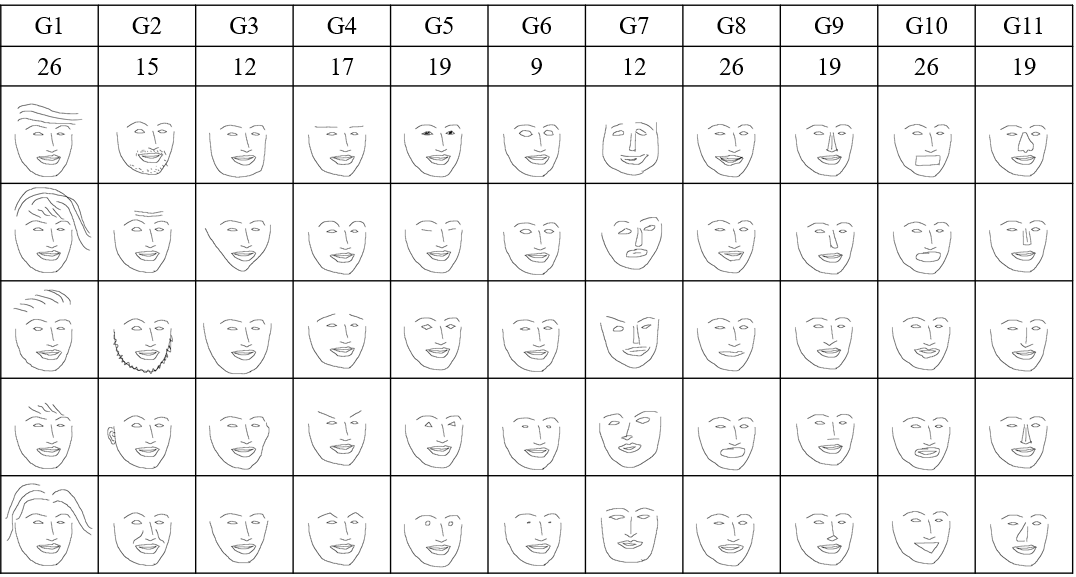
\includegraphics[width=0.9 \textwidth]{hand_drawn_sketches.png}
	\caption{These sketches can be divided into 11 categories. G1:Add hair; G2:Add new attributes, such as whiskers, wrinkles, ears; G3:Change face shape; G4:Change eyebrows; G5:Change eye shape; G6:changes eye size; G7:Graffiti-drawn; G8:Change mouth; G9:Change nose; G10:Change mouth(same eyes as G9); G11:Change nose(same eyes as G8). Specifically, there is no correlation between G7 and the other 10 categories. Except G7, the sketch in other categories only changes a particular area or attribute while the rest of the sketch remains the same. Except for the same eye between G8 and G11, G9 and G10, the eye lines of other categories of sketches are different.}
	\label{fig:hand_drawn_contours}
\end{figure*}

We refer to the first 5 layers of our generator as $L_0,\ldots,L_4$. 
With the hand-drawn sketch fed into the generator, we get 5 feature maps as output of $L_0$ to $L_4$, and then we extract one full channel feature vector on the left eye corner point of coordinate (170, 250) from each of the 5 feature maps respectively. 
We call the 5 vectors $\boldsymbol{v}_k,~k=0,\ldots,4$. 
The coordinates of the corresponding points on the five feature maps are (170, 250), (85, 125), (43, 63), (22, 32) and (11, 16). 
And the receptive fields of the 5 vectors are $7\times7$, $9\times9$,$13\times13$, $21\times21$ and $37\times37$ as shown in Fig.~\ref{fig:receptive}. 
The dimensions of these 5 feature vectors are 48, 96, 192, 384 and 768, respectively. 
We get the 5 feature vectors of pix2pixHD generator called $\boldsymbol{v}_0^{'},\ldots,\boldsymbol{v}_4^{'}$ in the same way.
\begin{figure}[htbp]
	\begin{center}
		%\centering
		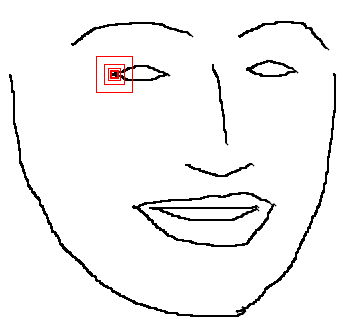
\includegraphics[width=0.2 \textwidth]{receptive_field.png}
	\end{center}
	\caption{The receptive fields of corresponding left eye corner points in the feature maps of $L_0\sim L_4$. }
	\label{fig:receptive}
\end{figure}

\noindent
$\mathbf{Visualization ~with ~PCA}$ Principal Component Analysis(PCA)\cite{pca} is a common linear data dimension reduction method, which can better retain the statistic characteristics of data in high dimensional space. 
We use PCA to perform visualization analysis on $\boldsymbol{v}_0\sim \boldsymbol{v}_4$ after dimension reduction.
Fig.~\ref{fig:pca_1}(a) and Fig.~\ref{fig:pca_1}(b) demonstrate the results of PCA visualization on $\boldsymbol{v}_0$ and $\boldsymbol{v}_1$. 
The corresponding relationship between hand-drawn sketch categories and number colors are: G1 (red), G2 (orange), G3 (lime), G4 (blue), G5 (cyan), G6 (magenta), G7 (maroon), G8 (olive), G9 (green), G10 (purple), G11 (teal). And it is applicable to the following sections.
It can be seen from the figure that the data of G1, G2, G3 and G4 are distributed at a same point separately, the data of G8 and G11 are gathered on the same point, the data of G9 and G10 are distributed at the same point, whereas the data of G5, G6 and G7 are distributed dispersedly. 
This indicates that after the removal of the instance normalization in the first two layers, the features of the left eye corner point are only affected by the contents of the sketch in the corresponding receptive field. The change of the sketch in the receptive field will influence the extracted features of the corresponding points but will not beyond the receptive field.
\begin{figure}[htb]
	\centering
	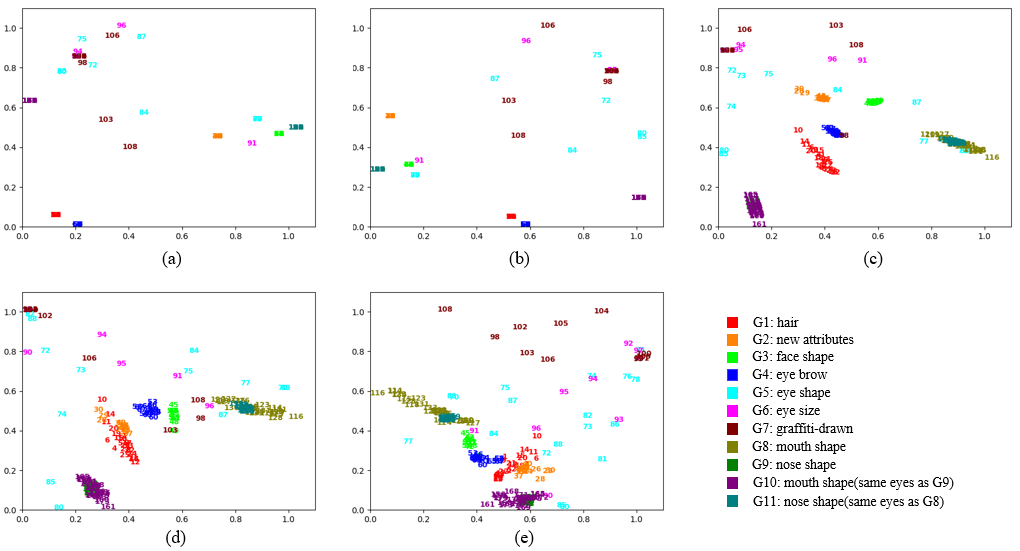
\includegraphics[width=0.47 \textwidth]{pca_1.png}
	\caption{Results of PCA visualization on $\boldsymbol{v}_0$ and $\boldsymbol{v}_1$}
	\label{fig:pca_1}
\end{figure}

Visualization results of $\boldsymbol{v}_2 \sim \boldsymbol{v}_4$ are shown in Fig.\ref{fig:pca_2}(a)(b)(c). 
By observing visualization results of $\boldsymbol{v}_2$, we can find out that the feature vectors belonging to categories with unmodified eyes have a different spatial distribution within class, which indicates that instance normalization conveys modification in other areas to left eye corner of sketches resulting in an effect on features extracted from left eye corner point. 
\begin{figure*}[htb]
	\centering
	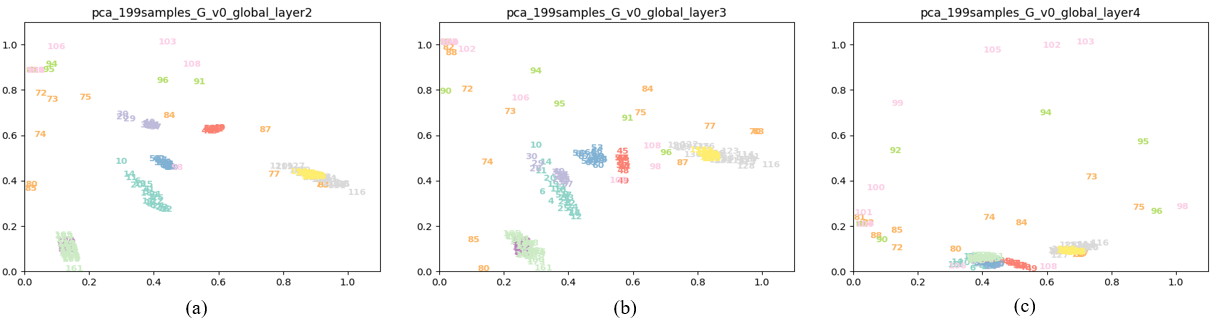
\includegraphics[width=0.8 \textwidth]{pca_2.png}
	\caption{PCA visualization results of $\boldsymbol{v}_2 \sim \boldsymbol{v}_4$}
	\label{fig:pca_2}
\end{figure*}
By comparing visualization results of $\boldsymbol{v}_2$ and $\boldsymbol{v}_4$, we can find out that the feature vectors belonging to categories with unmodified eyes such as G1, G2, G3, G4, G8, G9, G10, G11, distribute more and more dispersedly within class, which indicates that with the instance normalization operating layer by layer, changing other parts on the input sketch has more and more obvious influence on the features of the eye position, leading to the change of eyes in the generated image.

We also contrast the PCA visualization results of $\boldsymbol{v}_2 \sim \boldsymbol{v}_4$ and $\boldsymbol{v}_2^{'} \sim \boldsymbol{v}_4^{'}$ respectively. 
Fig.\ref{fig:pca_4}(a)(b)(c) illustrate the visualization results of $\boldsymbol{v}_2 \sim \boldsymbol{v}_4$, and Fig.\ref{fig:pca_4}(d)(e)(f) illustrate the visualization results of $\boldsymbol{v}_2^{'} \sim \boldsymbol{v}_4^{'}$. 
The $\boldsymbol{v}_2^{'}, \boldsymbol{v}_3^{'}, \boldsymbol{v}_4^{'}$ belonging to categories with unmodified eyes such as G1, G2, G3, G4, G8, G9, G10, G11, have a bigger in-class distance compared with $\boldsymbol{v}_2, \boldsymbol{v}_3, \boldsymbol{v}_4$. 
This exactly shows the removal of the first two instance normalization layers in pix2pixHD generator can better extract the low-level features of the input sketch, which can effectively reduce the influence of changing one part of the sketch on other parts of the generated image, and enhance fine-grained control on the generated images.
\begin{figure*}[htb]
	\centering
	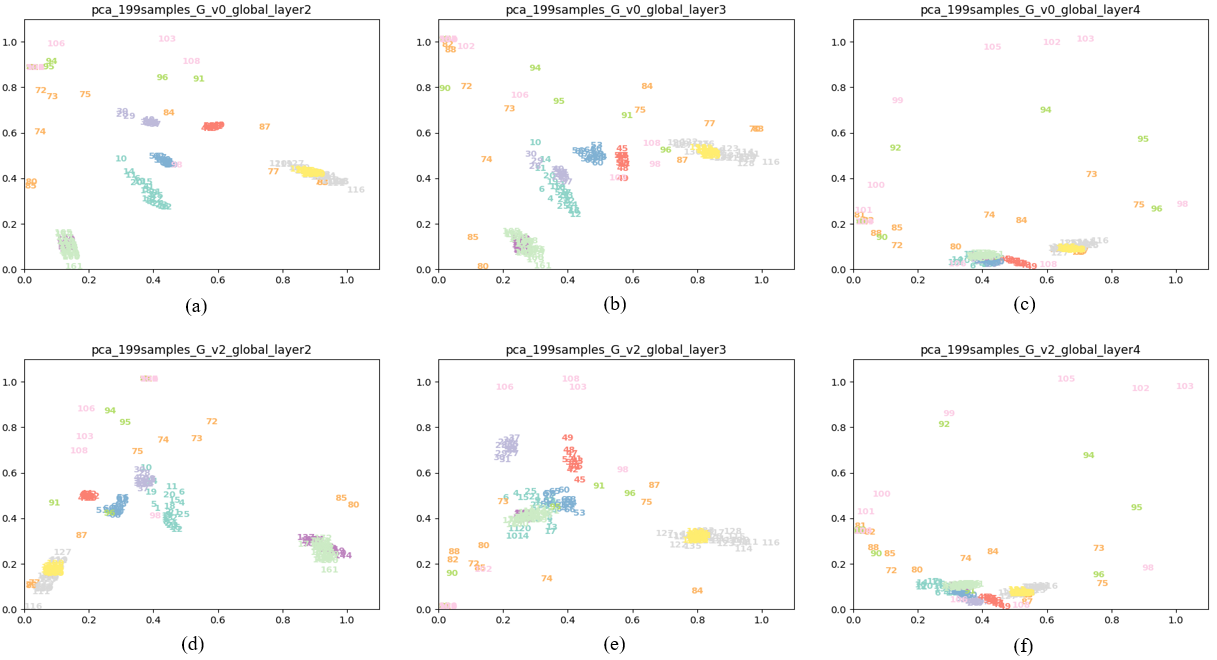
\includegraphics[width=0.8 \textwidth]{pca_4.png}
	\caption{Comparative PCA visualization results of $\boldsymbol{v}_2 \sim \boldsymbol{v}_4$ and $\boldsymbol{v}_2^{'} \sim \boldsymbol{v}_4^{'}$}
	\label{fig:pca_4}
\end{figure*}


\subsection{Network Architecture}\label{sec:network}
In baseline generator, the activation of convolutional output is normalized in the channel-wise manner and then modulated with unified scale and bias within channel. 
This operation, to a certain extent, leads to a negative effect that a local change in the input sketch broadcasts globally, thus resulting in a degraded capacity of fine-grained control on generated image.
 
However, the vanishing gradient or exploding gradient problem is bound to emerge when the instance normalization layers in feature extraction stage of the generator network is abandoned too much, which makes the training process difficult to converge. 
Based on the consideration above, we remove the first two instance normalization layers in the global generator of pix2pixHD baseline and take the rest as our own generator. 
The architecture of our generator is shown in Fig.\ref{fig:our_generator}. And it operates at a resolution of 512×512. 
It consists of four components: a convolutional front-end without normalization $G_1^{(F)}$, a down-sampled convolutional mid-end $G_1^{(M)}$, a set of residual blocks $G_1^{(R)}$ and a transposed convolutional back-end $G_1^{(B)}$. 
$G_1^{(F)}$ composed of two unnormalized convolution and activation layers can remain underlying information of input sketches locally, in other words, semantic information flows through the network without spatially broadcasting. 
Hence efficient fine-grained control on generated images can be conduct. %we use the global generator of pix2pixHD baseline without the first two instance normalization layers as our own generator.%
\begin{figure*}[htbp]
	\centering
	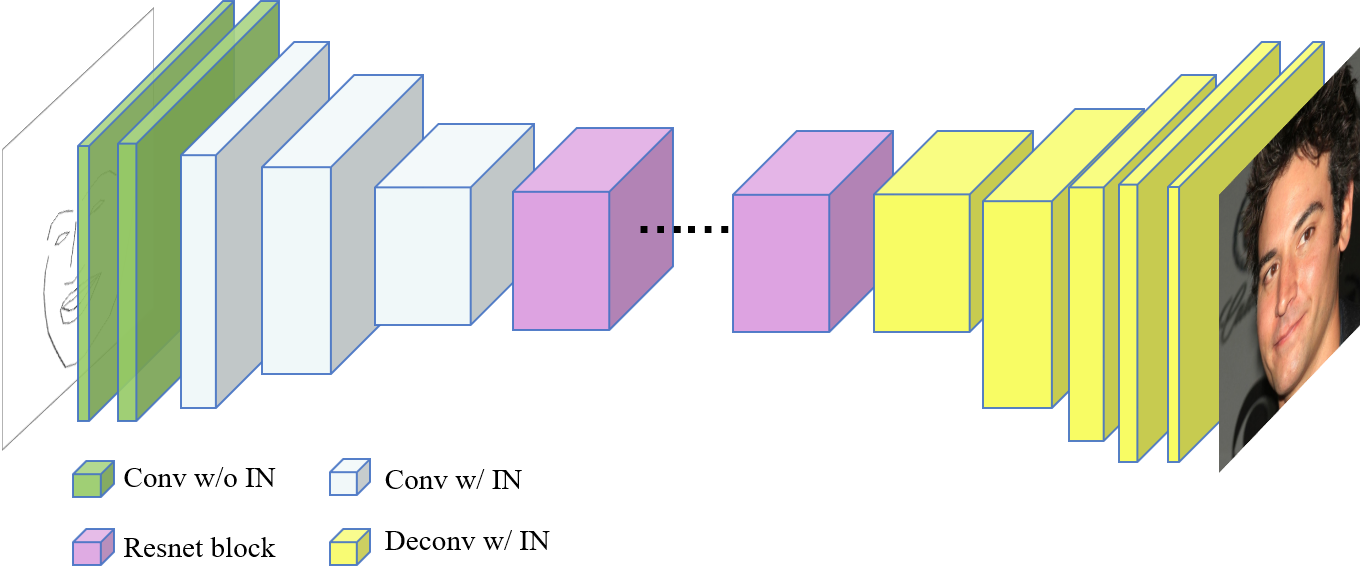
\includegraphics[width=0.8 \textwidth]{our_model_G.png}
	\caption{Network architecture of our generator. }
	\label{fig:our_generator}
\end{figure*}

The discriminator applys the multi-scale design consistent with pix2pixHD. 
There are three discriminators that have an identical network structure but operate at different image scales. 
In addition, each discriminator is built on PatchGAN\cite{pix2pix} architecture proposed by Isola Phillip \textit{et al.}. Sketches at different scales are concatenated with corresponding face images, and fed into the discriminators, respectively. 


\section{Experiments}
We conduct extensive experiments to evaluate our proposed method.
In Sec.~\ref{sec:datasets}, we introduce how to produce our training and testing datasets(). 
In Sec.~\ref{sec:augmentation}, we introduce the method of data augmentation aiming to alleviate the issue that the generated image has poor tolerance to the spatial position change of the input sketches. And we show the generation results of the model trained with augmented data. 
In Sec.~\ref{sec:results}, we conduct comparative experiments on hand-drawn sketches between our methods and pix2pixHD baseline. We show that our method achieves a better fine-grained control on generated images.

\subsection{Datasets}\label{sec:datasets} 
CelebA-HQ dataset contains more than 30,000 face images generated by PGGAN\cite{pggan} of resolution 1024×1024. Since the images are cropped according to face landmarks, each image is global aligned. 
We extracted 68 landmarks from the face images in the CelebA-HQ dataset, and then connected these points in sequence with a line of pixel 2 to form the contour. As the face photos in Celeba-HQ dataset are global aligned, so are the contours. Contour is more simple and clean than other types of sketch like edge maps\cite{csagan} and mask edge maps\cite{maskgan}, so it is more suitble to imitate human hand-drawn sketch. Therefore, it is more reasonable to use contour as training data.
For the purpose of the experiment, we scaled the picture of resolution 512×512. After selection, the training set contains 14,973 pairs of contour and face photos, while the test set contains 4,992 pairs of contour and face photos. 
In order to evaluate the generalization ability of our model on the hand-drawn sketches, we develop an interactive interface for drawing sketches and displaying the generated photos in real time.

\subsection{Data Augmentation}\label{sec:augmentation} 
Since the face photos of the CalebA-HQ dataset are cropped with the reference of facial landmarks, and our training data contours are also obtained based on facial landmarks, we intuitively believe that all the facial landmarks of the training data have spatial consistency. 
To verify the hypothesis above, we calculate the average face of all the training data, as shown in Fig.\ref{fig:average_face}. We find that the facial features and facial contours of training data are basically in the same position, in other words, the training data is global aligned. This issue leads to degraded generalization ability of the model. 
\begin{figure}[htb]
	\centering
	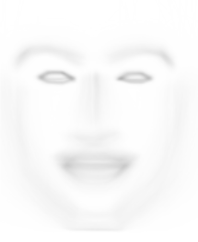
\includegraphics[width=0.18 \textwidth]{average_face.png}
	\caption{The average face of all the training data. }
	\label{fig:average_face}
\end{figure}
In order to imitate the human hand-drawn sketches, we apply random translation and rotation to the training contours. Specifically, offsets randomly selected from $[-d,d]^2$ and angles randomly selected from $[-\theta,\theta]$ are added to the training contours, where $d$ is the maximum offset and $\theta$ is the maximum angle and we set $d=25$, $\theta=7^\circ$ in our experiments. 
But face photos are not translated or rotated because we expect the generated images to remain global aligned regardless of the spatial location of the input sketches.
Fig.\ref{fig:data_augmentation} illustrates the comparisons between images generated before data augmentation and  that after data augmentation. 
\begin{figure}[htb]
	\centering
	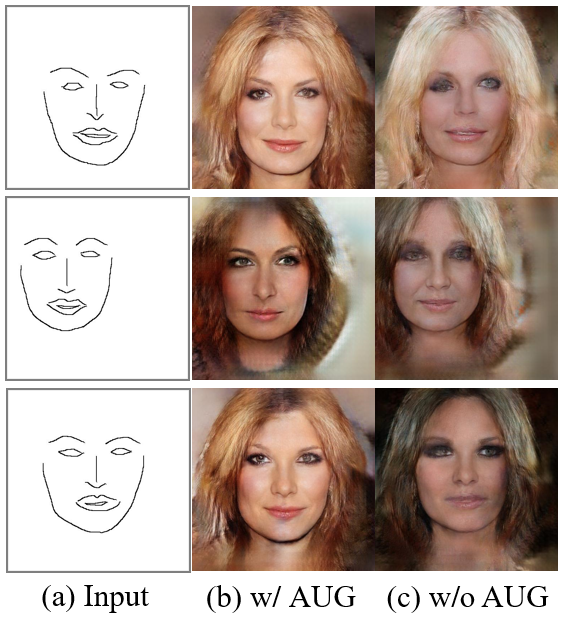
\includegraphics[width=0.35 \textwidth]{data_augmentation.png}
	\caption{Comparison between images generated before and after data augmentation. The quality of generated images after data augmentation is better than that before data augmentation when the inputs deviate from standard position.}
	\label{fig:data_augmentation}
\end{figure}

\subsection{Qualitatively Comparisons}\label{sec:results}
As you can see in Fig.\ref{fig:ablation}, our model generates the most photorealistic images in contrast to the $M_2$ model producing images with lowest sense of reality. It indicates that removing too many instance normalization layers in generator can weaken the model as reason of gradient vanishing.
\begin{figure}[htb]
	\centering
	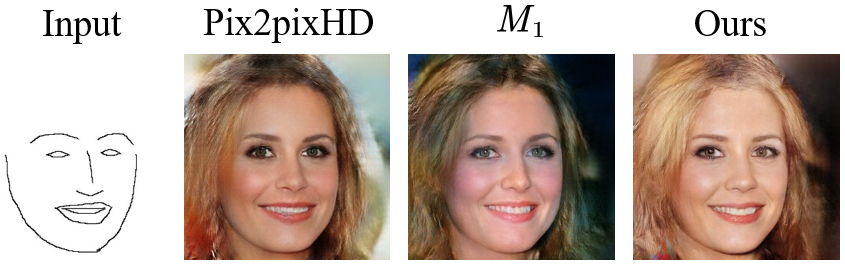
\includegraphics[width=0.5 \textwidth]{ablation.png}
	\caption{Comparison on amount of instance normalization layers. We refer to original pix2pixHD model as $M_1$, refer to the model of which generator gets rid of first 5 IN layers as $M_2$.}
	\label{fig:ablation}
\end{figure}  

We perform comparative experiments between our model and pix2pixHD baseline on hand-drawn sketches.
Results shown in Fig.\ref{fig:compare_1} demonstrate that the baseline model frequently fails to produce realistic textures. In contrast, our results are more realistic with fine textures.  
\begin{figure}[htb]
	\centering
	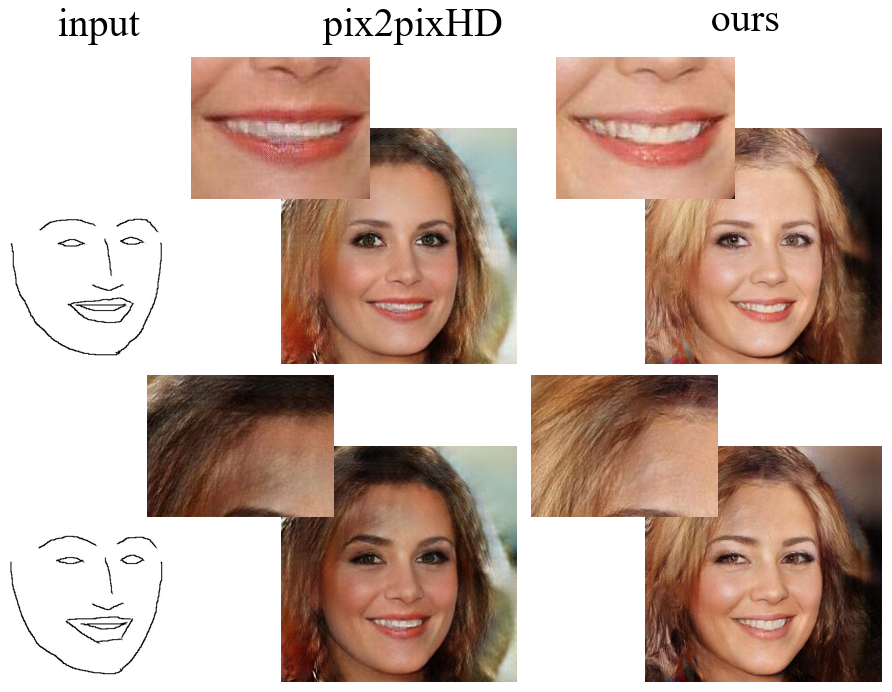
\includegraphics[width=0.45 \textwidth]{texture.png}
	\caption{Magnified details of images generated by our model and baseline model. The top row shows that the textures of teeth generated by pix2pixHD baseline are blurry, while our results have clear textures of teeth. The bottom row shows that some chaotic noises often emerge in the forehead of images generated by pix2pixHD baseline, but our results do not have this issue.}
	\label{fig:compare_1}
\end{figure}

Our model can achieve fine-grained control on generated images, whereas baseline model cannot. When we modify the lines of face parts or face shapes of input freehand sketches, the corresponding parts of images generated by our model change simultaneously but other areas remain unchanged. 
In comparison, modifying strokes of sketches influences not only the content in corresponding areas of images generated by baseline model but also the content in other areas. 
Fig.\ref{fig:compare_2} and Fig.\ref{fig:compare_3}~ show several face images generated by our model and baseline model when changing lines of mouth and nose separately in sketches.
The results shown in row 1, 2 of Fig.\ref{fig:compare_2} demonstrate that the images generated by our model change obviously in mouth shape and preserve structure conformance with input sketches when modifying the lines of mouth in sketches. But the results generated by baseline model do not have an obvious change in mouth shape.
The results shown in Fig.\ref{fig:compare_3} illustrate that the images generated by our model remain unchanged in other areas especially in eyes when altering the shapes of nose in sketches, but the images generated by baseline model change obviously in eyes direction. And as shown in row 3 of Fig.\ref{fig:compare_2}, the generation results of our model do not change except the mouth when modifying the mouth shape in sketches, while the generation quality of baseline model is degraded vastly especially in the eye area. 
\begin{figure}[htb]
	\centering
	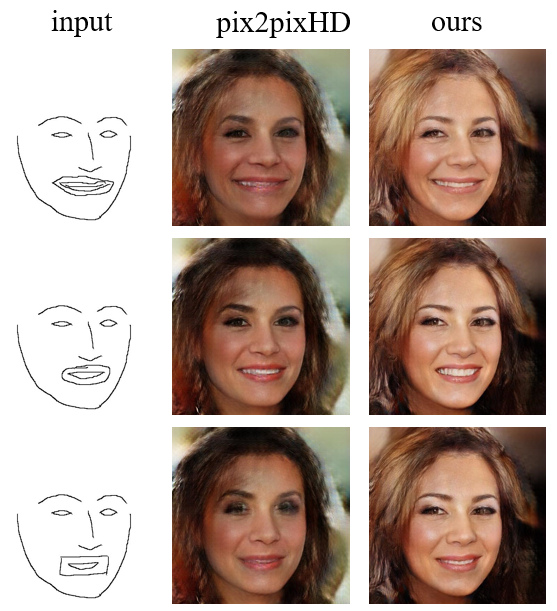
\includegraphics[width=0.4 \textwidth]{mouth_editing.png}
	\caption{Comparison between our model and baseline model tested with mouth-altered sketches. }
	\label{fig:compare_2}
\end{figure}

\begin{figure}[htb]
	\centering
	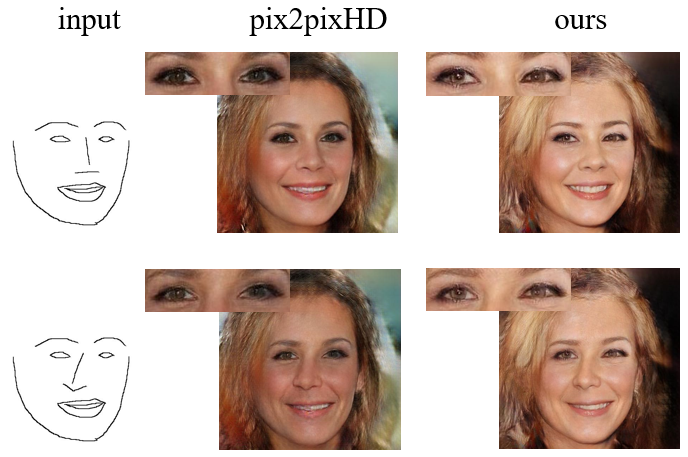
\includegraphics[width=0.45 \textwidth]{nose_editing.png}
	\caption{Comparison between our model and baseline model tested with nose-altered sketches.}
	\label{fig:compare_3}
\end{figure}

\section{Conclusion}
In this paper, we utilize PCA, a visualization approach to analyze the feature embedding for sketches with a group of specific changes.  
Then we modify the baseline image translation model by removing the first two instance normalization layers in its generator. 
We show the effectiveness of the proposed simple modification in the generator architecture on making a significant improvement of the image generation quality and conformance with user intention. 
User studies demonstrate that our method surpass the baseline method regarding both face editing and image fidelity.    


%\section{About the paper submission}
%
%\subsection{Paper length}
%cvm papers may be between 4 pages and 14 pages. Over length papers will simply not be reviewed.
%
%%-------------------------------------------------------------------------
%\subsection{Draft and final copy}
%The \LaTeX\ style defines a printed ruler which should be present in the
%version submitted for review.  The ruler is provided in order that
%reviewers may comment on particular lines in the paper without
%circumlocution. The camera ready copy should not contain a ruler.
%(\LaTeX\ users may uncomment the \verb'\cvmfinalcopy' command in the document preamble.)
%
%\subsection{Blind review}
%Many authors misunderstand the concept of anonymizing for blind
%review.  Blind review does not mean that one must remove
%citations to one's own work---in fact it is often impossible to
%review a paper unless the previous citations are known and
%available.
%Blind review means that you do not use the words ``my'' or ``our''
%when citing previous work.
%
%%\begin{figure}[t]
%%\begin{center}
%%\fbox{\rule{0pt}{2in} \rule{0.9\linewidth}{0pt}}
%%   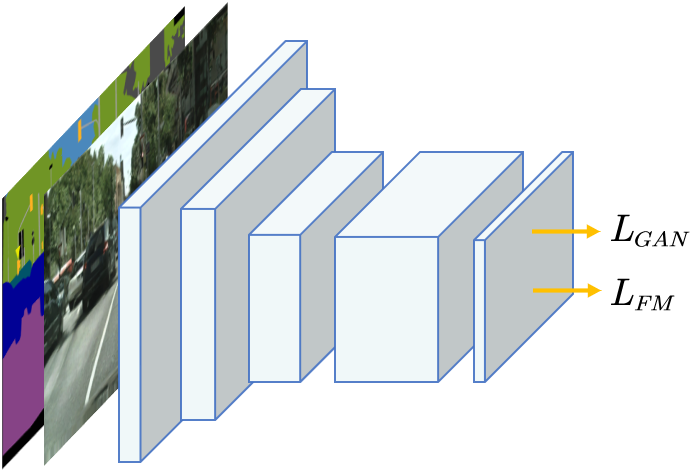
\includegraphics[width=0.8\linewidth]{pix2pixhd_D.png}
%%\end{center}
%%   \caption{Example of caption. }
%%\label{fig:long}
%%\label{fig:onecol}
%%\end{figure}
%
%\subsection{Miscellaneous}
%
%\noindent
%Compare the following:\\
%\begin{tabular}{ll}
% \verb'$conf_a$' &  $conf_a$ \\
% \verb'$\mathit{conf}_a$' & $\mathit{conf}_a$
%\end{tabular}\\
%See The \TeX book, p165.
%
%The space after \eg, meaning ``for example'', should not be a
%sentence-ending space. So \eg is correct, {\em e.g.} is not.  The provided
%\verb'\eg' macro takes care of this.
%
%When citing a multi-author paper, you may save space by using ``et alia'',
%shortened to ``\etal'' (not ``{\em et.\ al.}'' as ``{\em et}'' is a complete word.)
%However, use it only when there are three or more authors.  Thus, the
%following is correct: ``
%   Frobnication has been trendy lately.
%   It was introduced by Alpher~\cite{Alpher02}, and subsequently developed by
%   Alpher and Fotheringham-Smythe~\cite{Alpher03}, and Alpher \etal~\cite{Alpher04}.''
%
%This is incorrect: ``... subsequently developed by Alpher \etal~\cite{Alpher03} ...''
%because reference~\cite{Alpher03} has just two authors.  If you use the
%\verb'\etal' macro provided, then you need not worry about double periods
%when used at the end of a sentence as in Alpher \etal.
%
%For this citation style, keep multiple citations in numerical (not
%chronological) order, so prefer \cite{Alpher03,Alpher02,Authors12} to
%\cite{Alpher02,Alpher03,Authors12}.
%
%%-------------------------------------------------------------------------
%\subsection{References}
%
%List and number all bibliographical references in 9-point Times,
%single-spaced, at the end of your paper. When referenced in the text,
%enclose the citation number in square brackets, for
%example~\cite{Authors12}.  Where appropriate, include the name(s) of
%editors of referenced books.
%
%\begin{table}
%\begin{center}
%\begin{tabular}{|l|c|}
%\hline
%Name & Performance \\
%\hline\hline
%A & OK\\
%B & Bad \\
%Ours & Great\\
%\hline
%\end{tabular}
%\end{center}
%\caption{An example for using tables.}
%\end{table}
%
%%-------------------------------------------------------------------------
%\subsection{Illustrations, graphs, and photographs}
%
%All graphics should be centered.  Please ensure that any point you wish to
%make is resolvable in a printed copy of the paper.  Resize fonts in figures
%to match the font in the body text, and choose line widths which render
%effectively in print.  Many readers (and reviewers), even of an electronic
%copy, will choose to print your paper in order to read it.  You cannot
%insist that they do otherwise, and therefore must not assume that they can
%zoom in to see tiny details on a graphic.
%
%When placing figures in \LaTeX, it's almost always best to use
%\verb+\includegraphics+, and to specify the  figure width as a multiple of
%the line width as in the example below
%{\small\begin{verbatim}
%   \usepackage[dvips]{graphicx} ...
%   \includegraphics[width=0.8\linewidth]
%                   {myfile.eps}
%\end{verbatim}
%}
%
%
%%-------------------------------------------------------------------------
%
{\small
\bibliographystyle{cvm}
\bibliography{cvmbib}
}

\end{document}
